\section{Evaluation}
\label{sec:evaluation}

\subsection{Dataset}
We collected a dataset comprising of 149 stained tissue images in collaboration with pathologists. The images are taken at a magnification of $10\times$, and are all scaled to a resolution of $1000\times 1000$. Each image in the dataset has been marked as `cancerous' or `non-cancerous' by a pathologist. Some sample images from the dataset are shown in Figure~\ref{fig:TissueImageExample}.

\begin{figure}
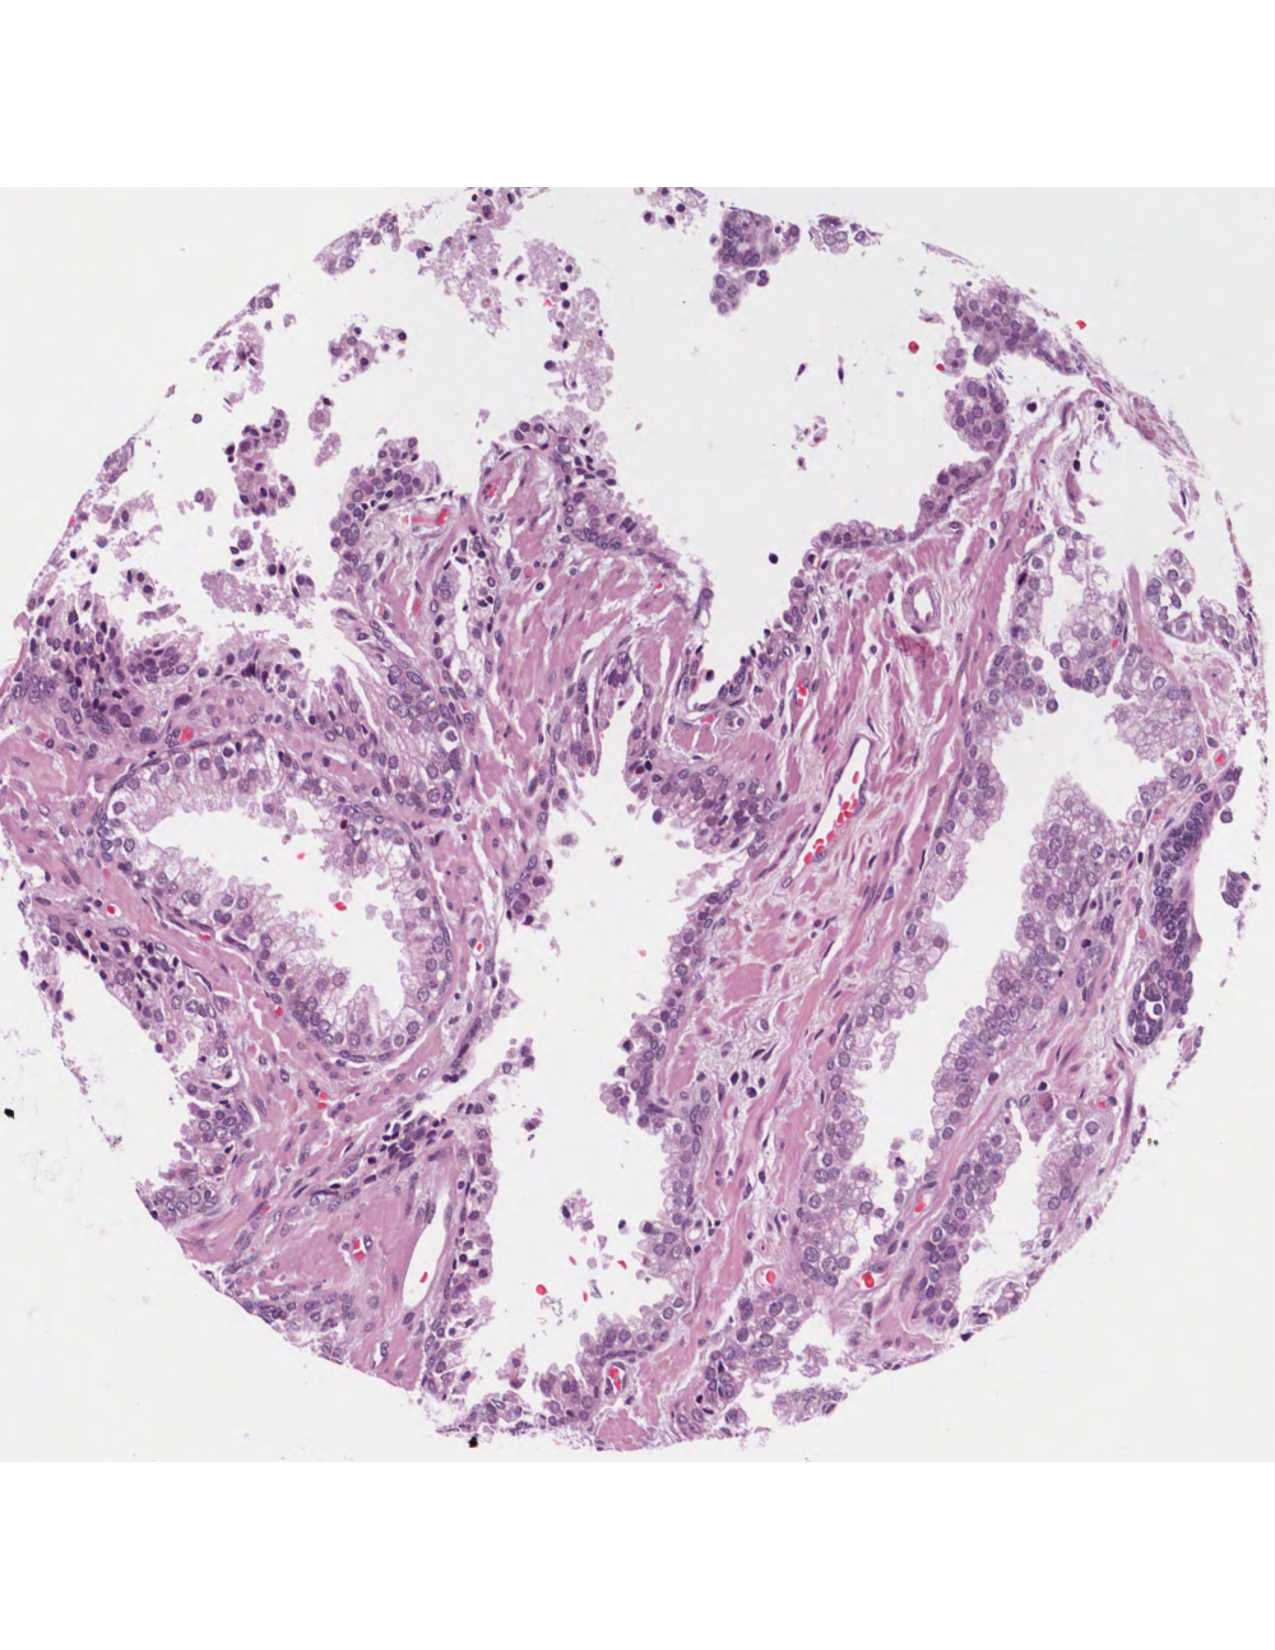
\includegraphics[width=2.0cm]{figs/145_green.pdf}
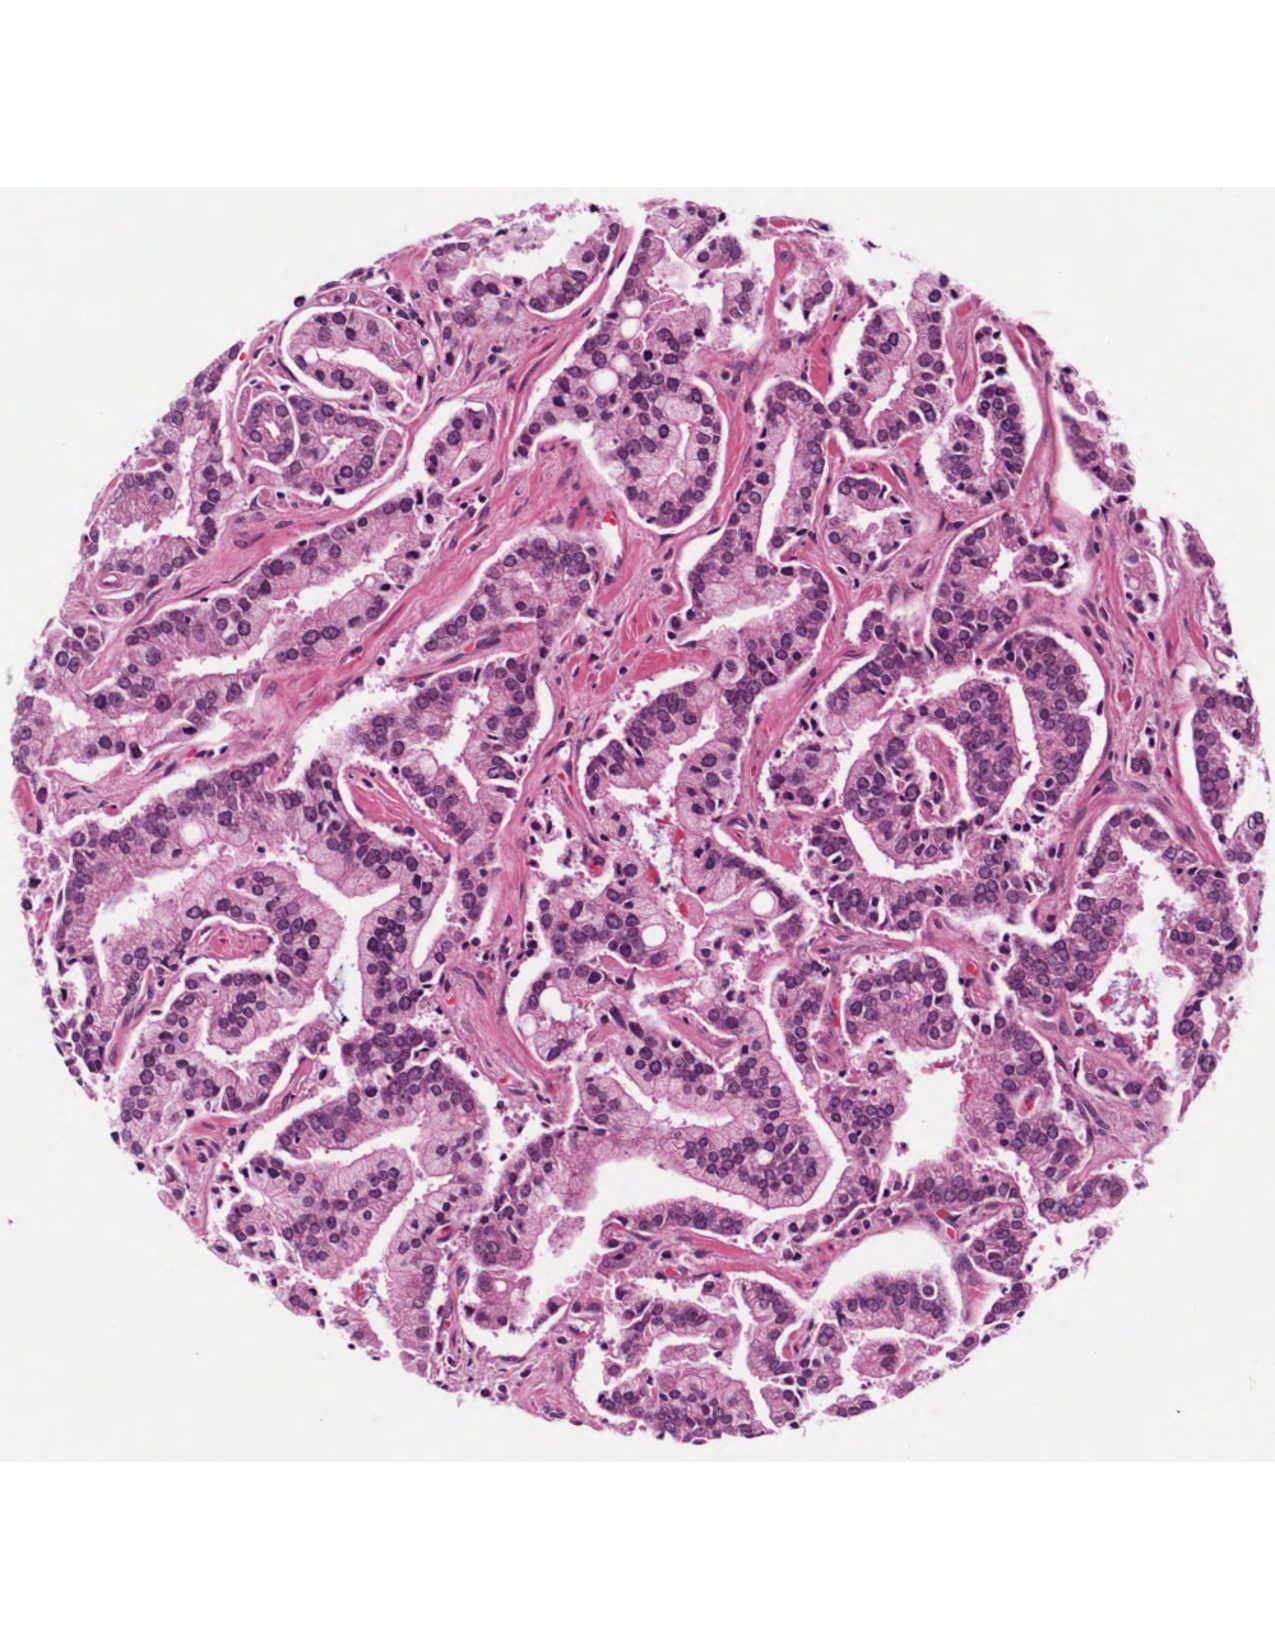
\includegraphics[width=2.0cm]{figs/93_red.pdf}
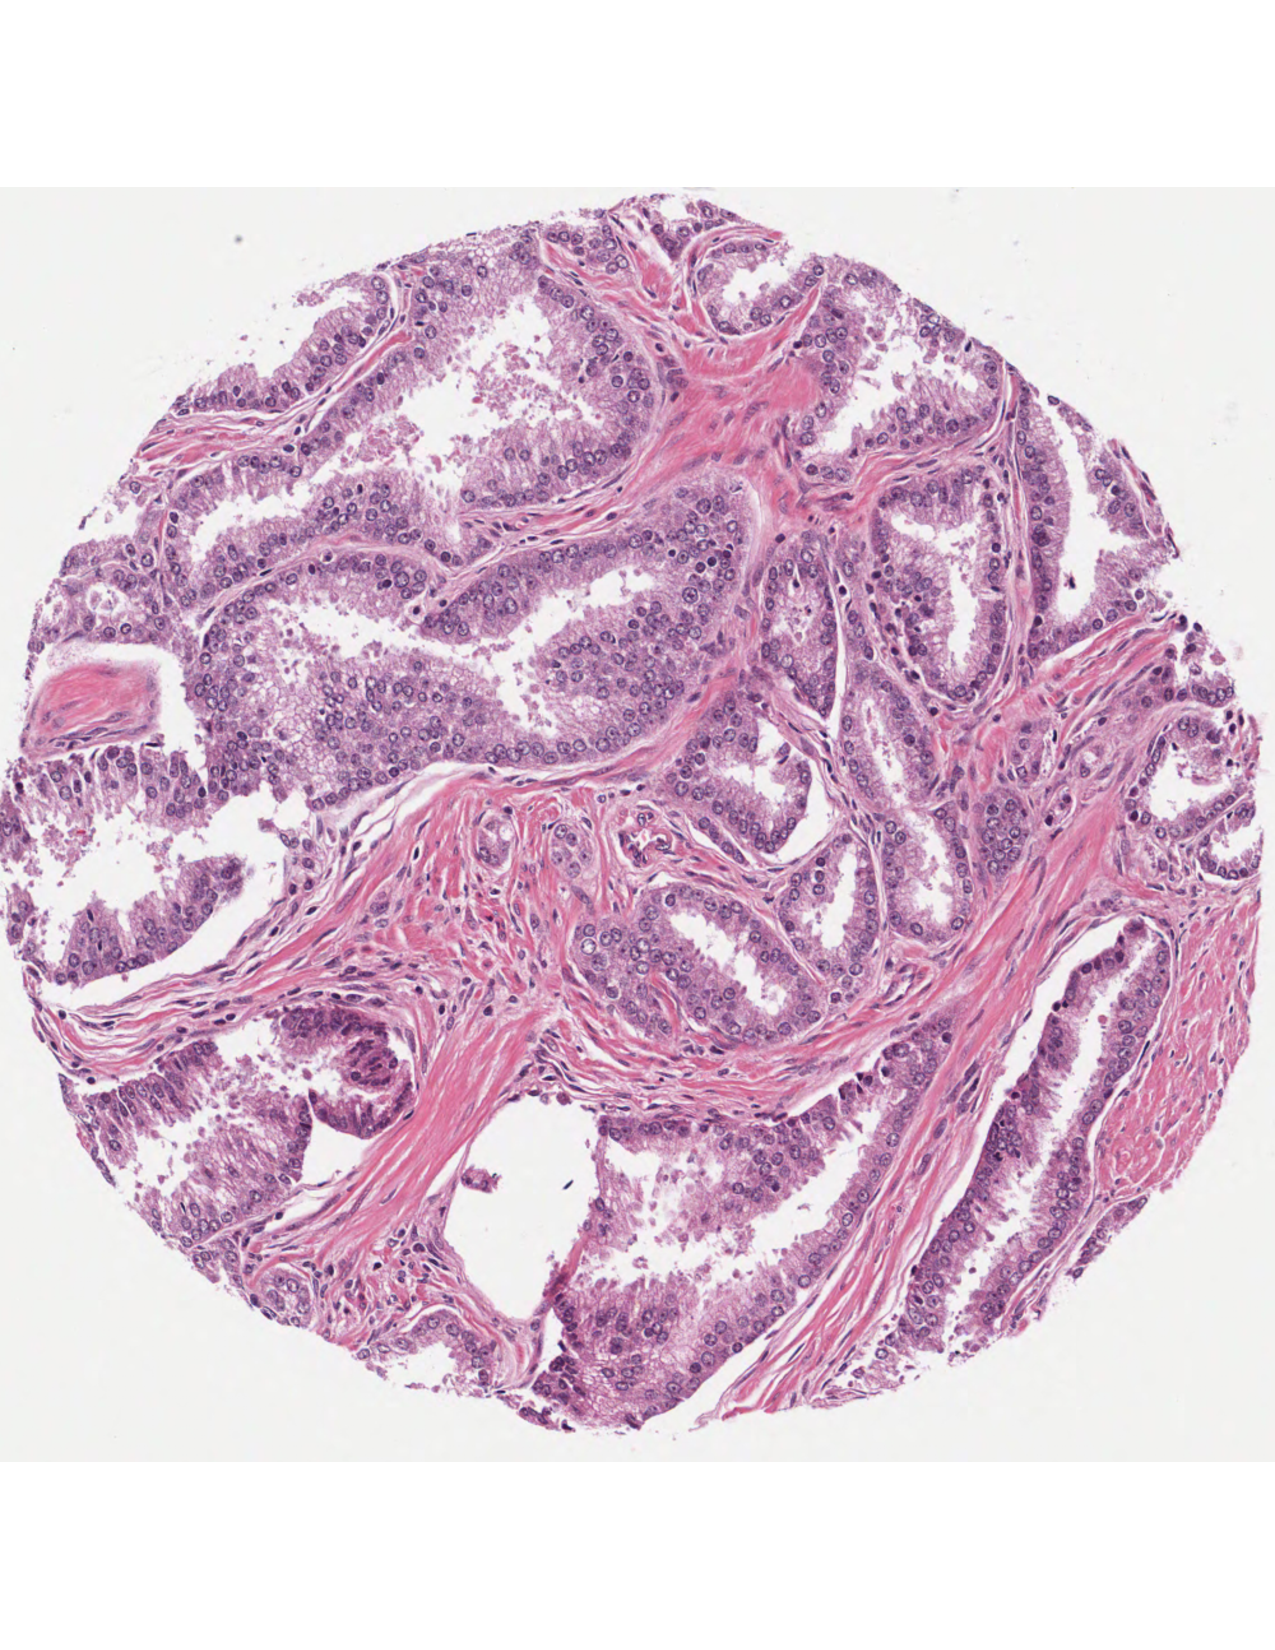
\includegraphics[width=2.0cm]{figs/130_green.pdf}
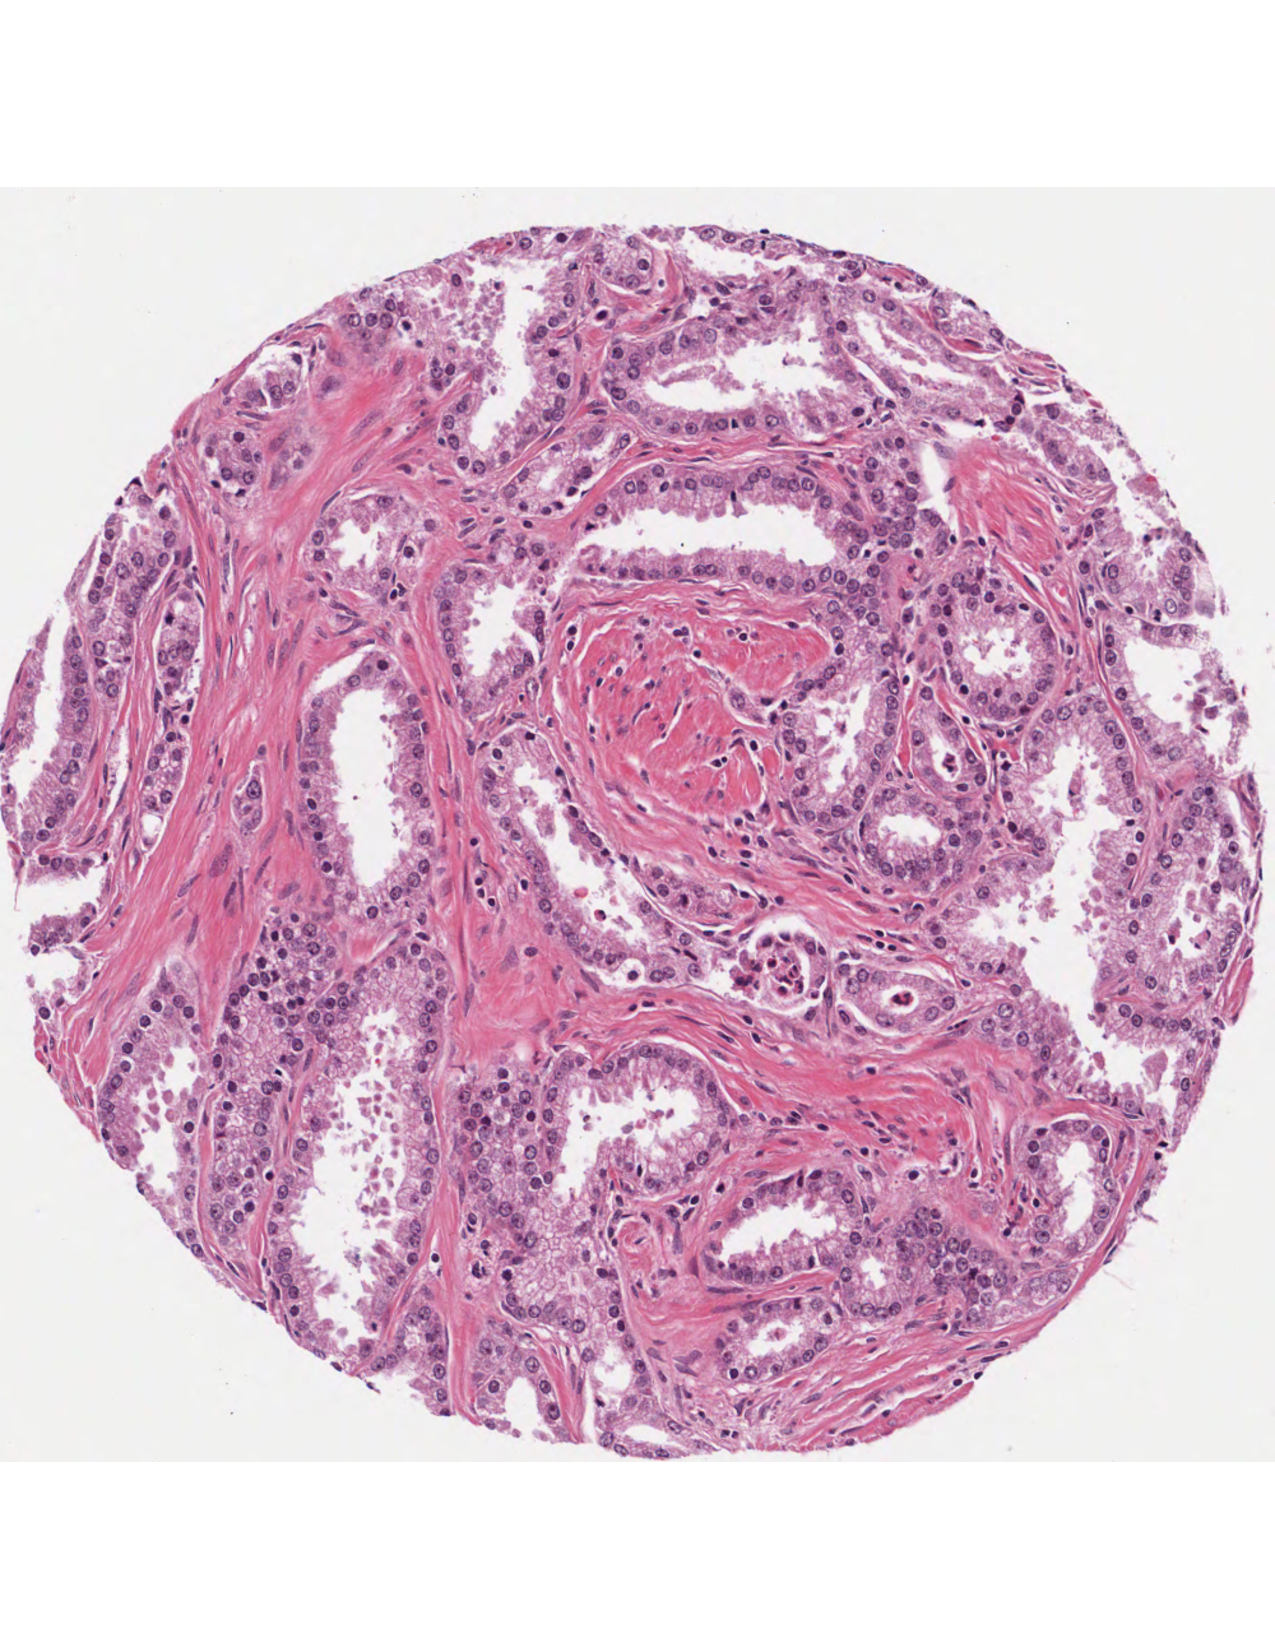
\includegraphics[width=2.0cm]{figs/87_red.pdf}
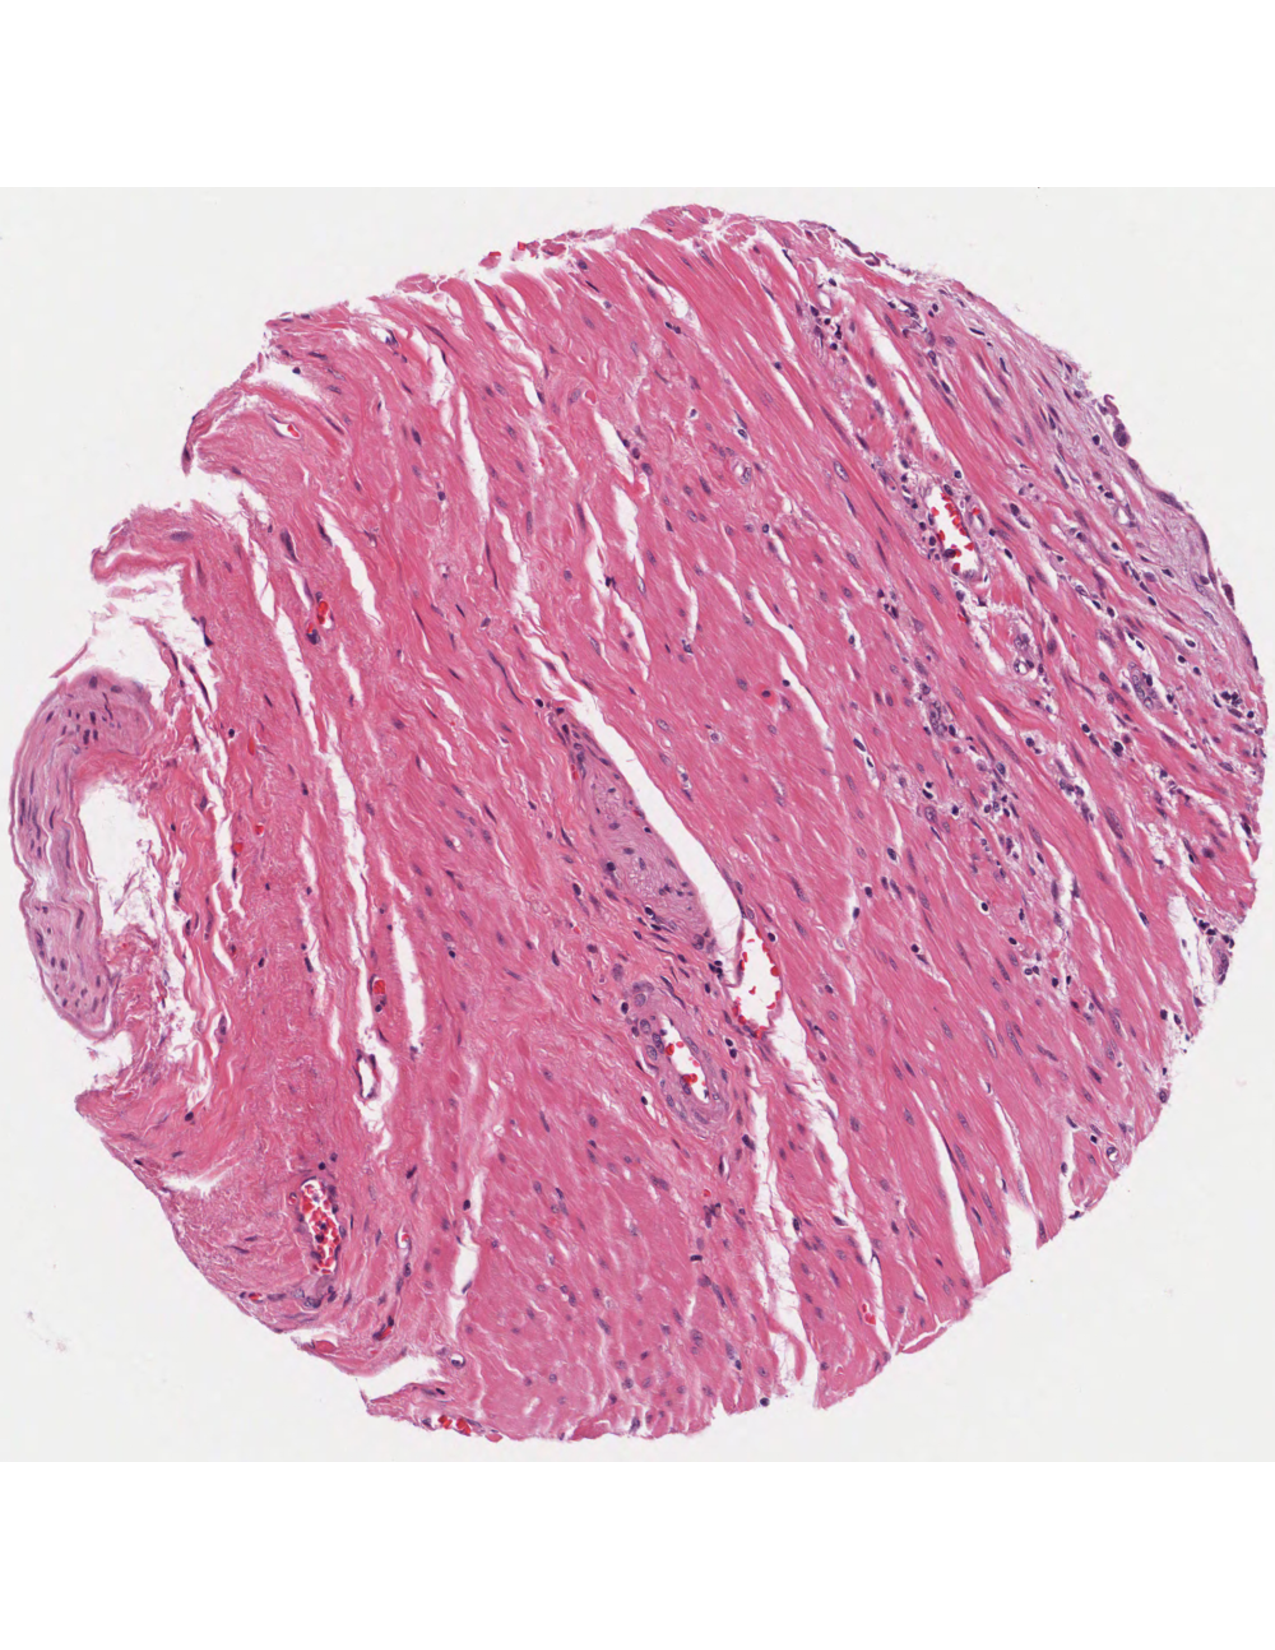
\includegraphics[width=2.0cm]{figs/63_green.pdf}
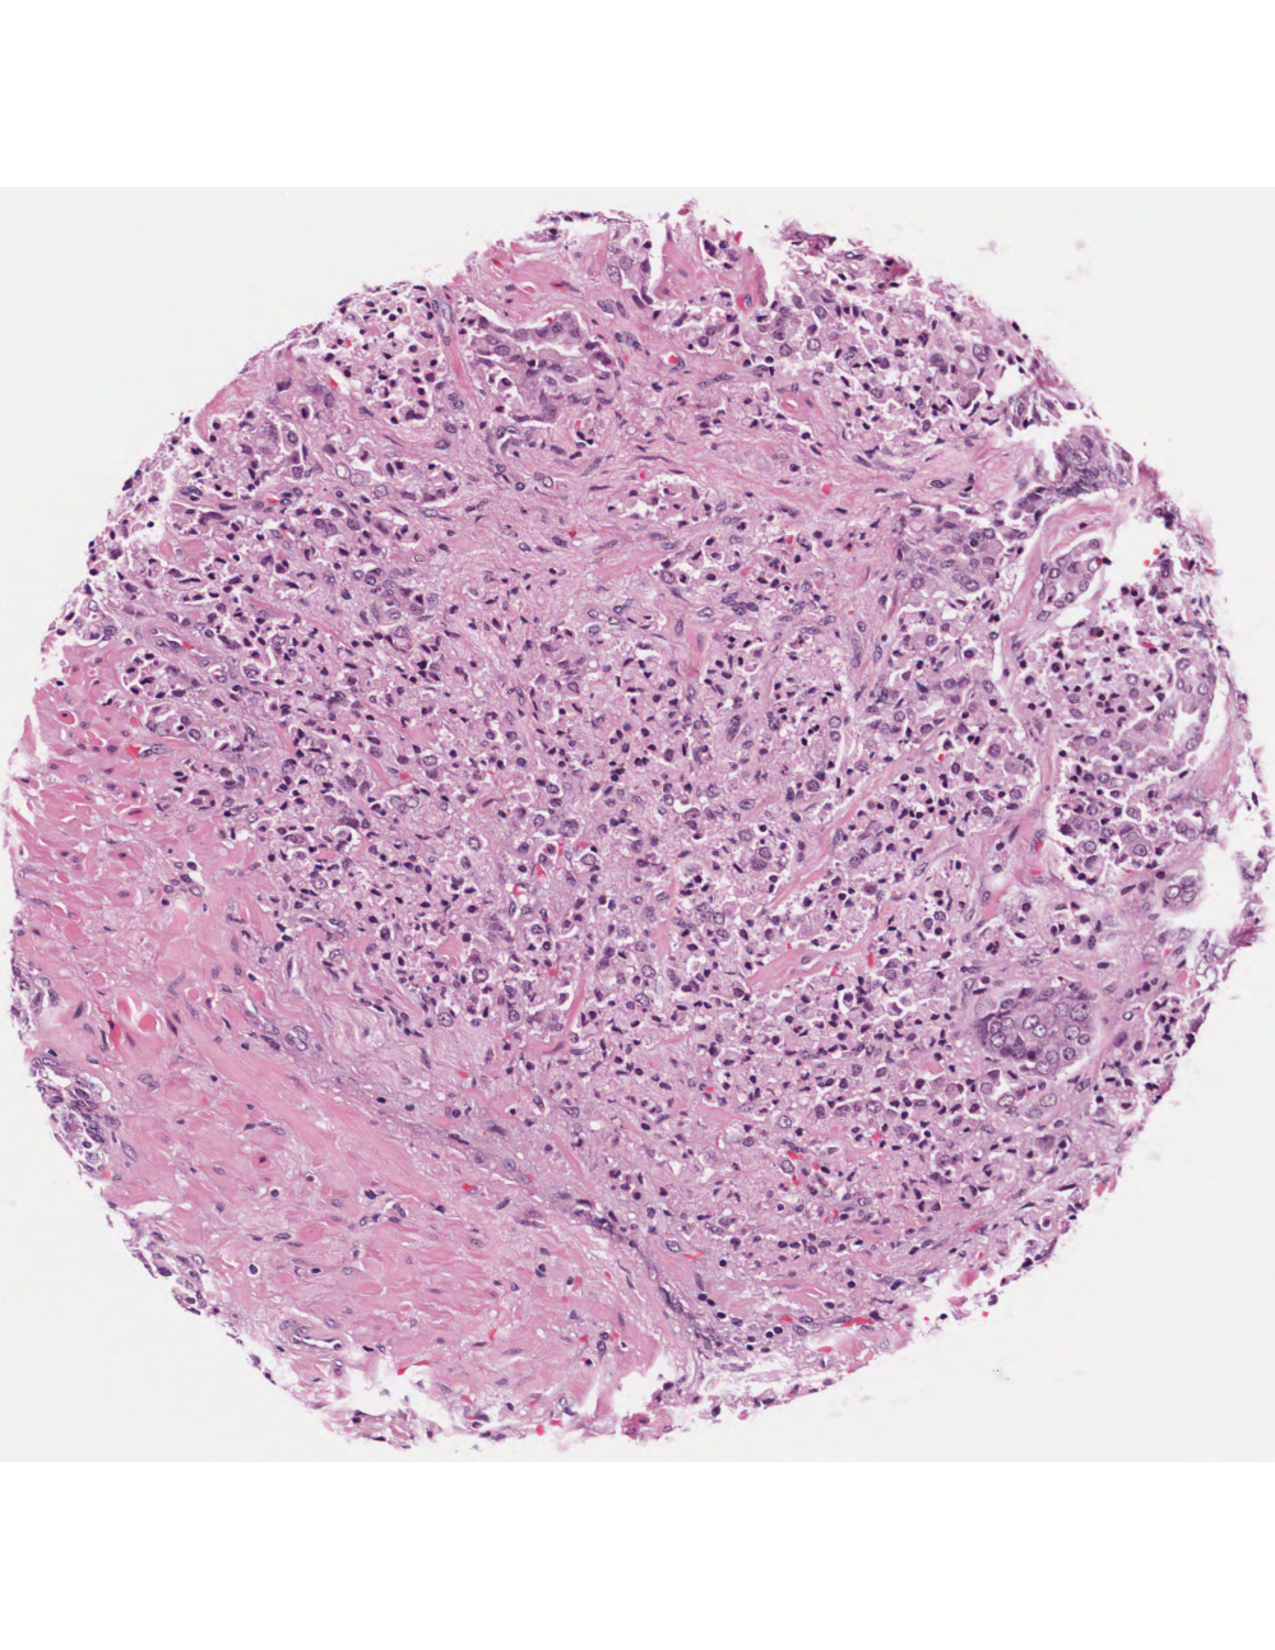
\includegraphics[width=2.0cm]{figs/41_red.pdf}
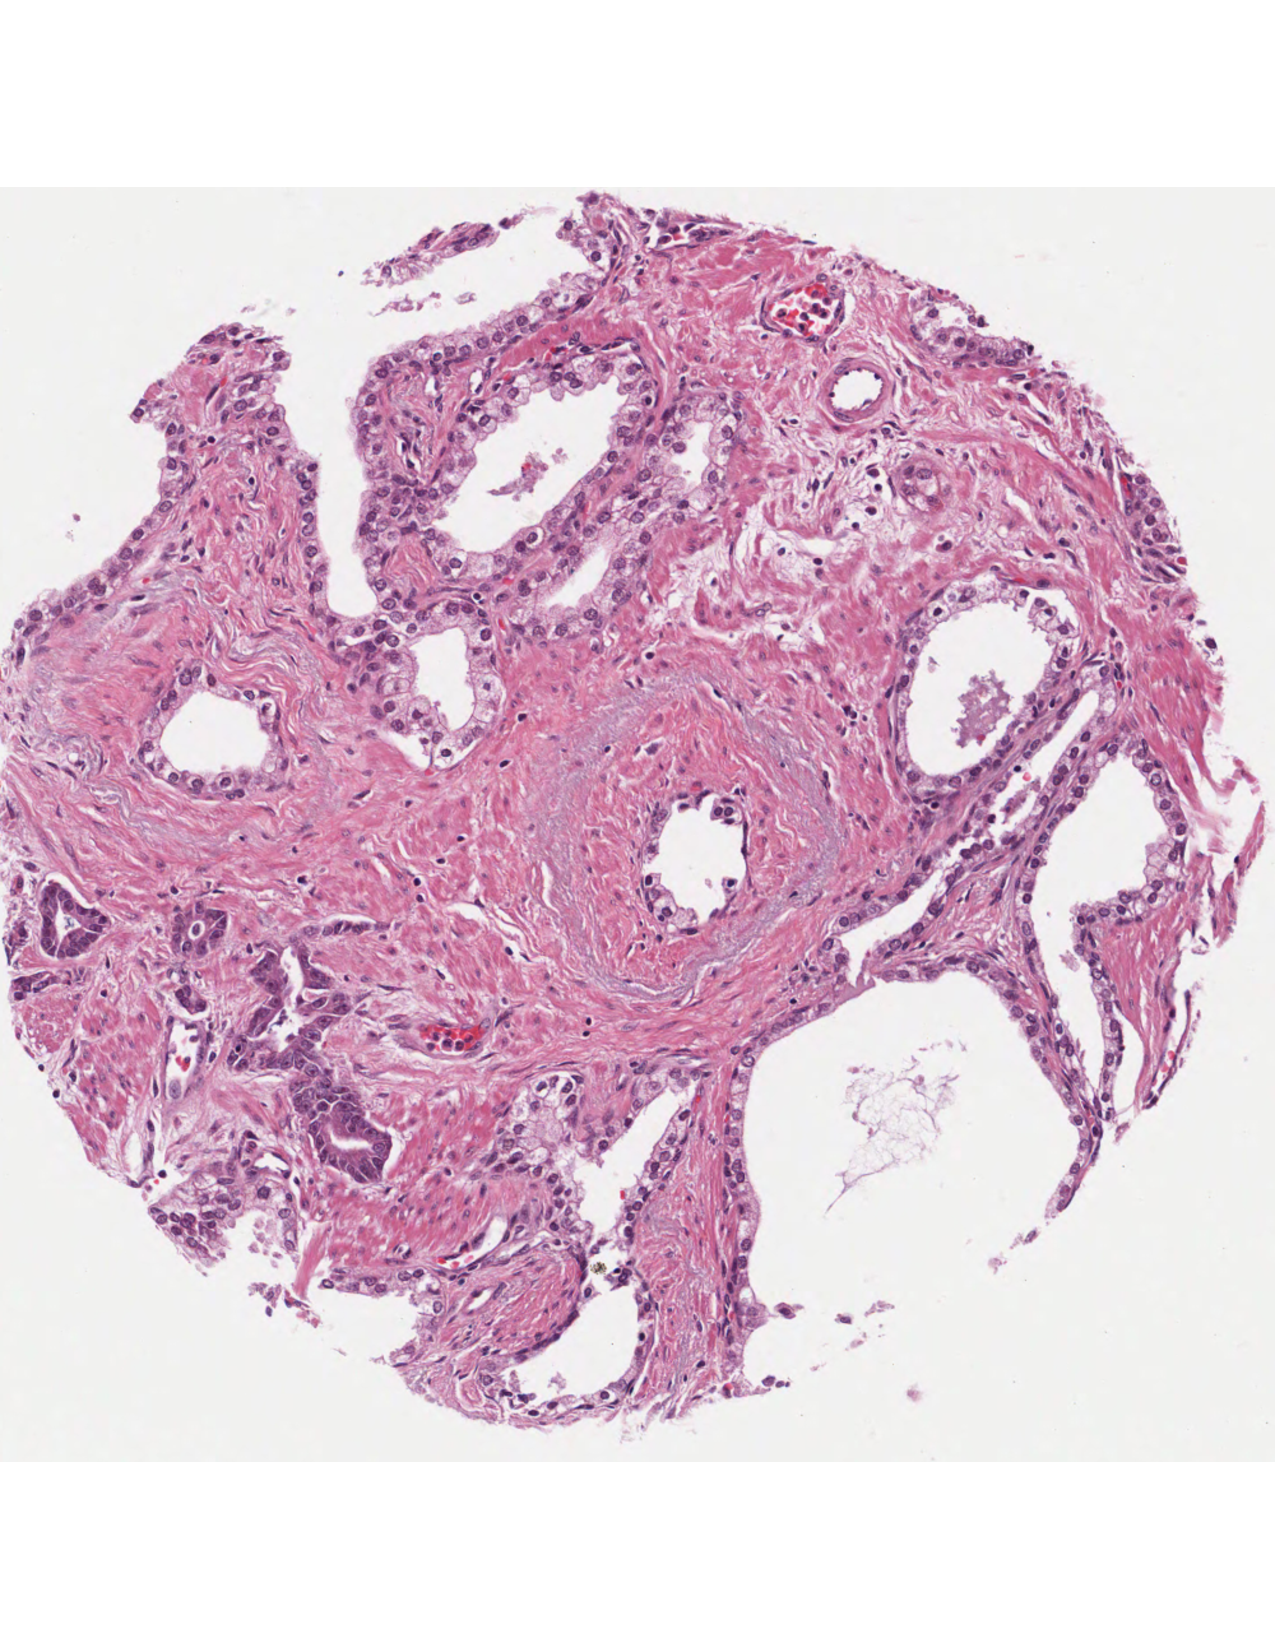
\includegraphics[width=2.0cm]{figs/108_green.pdf}
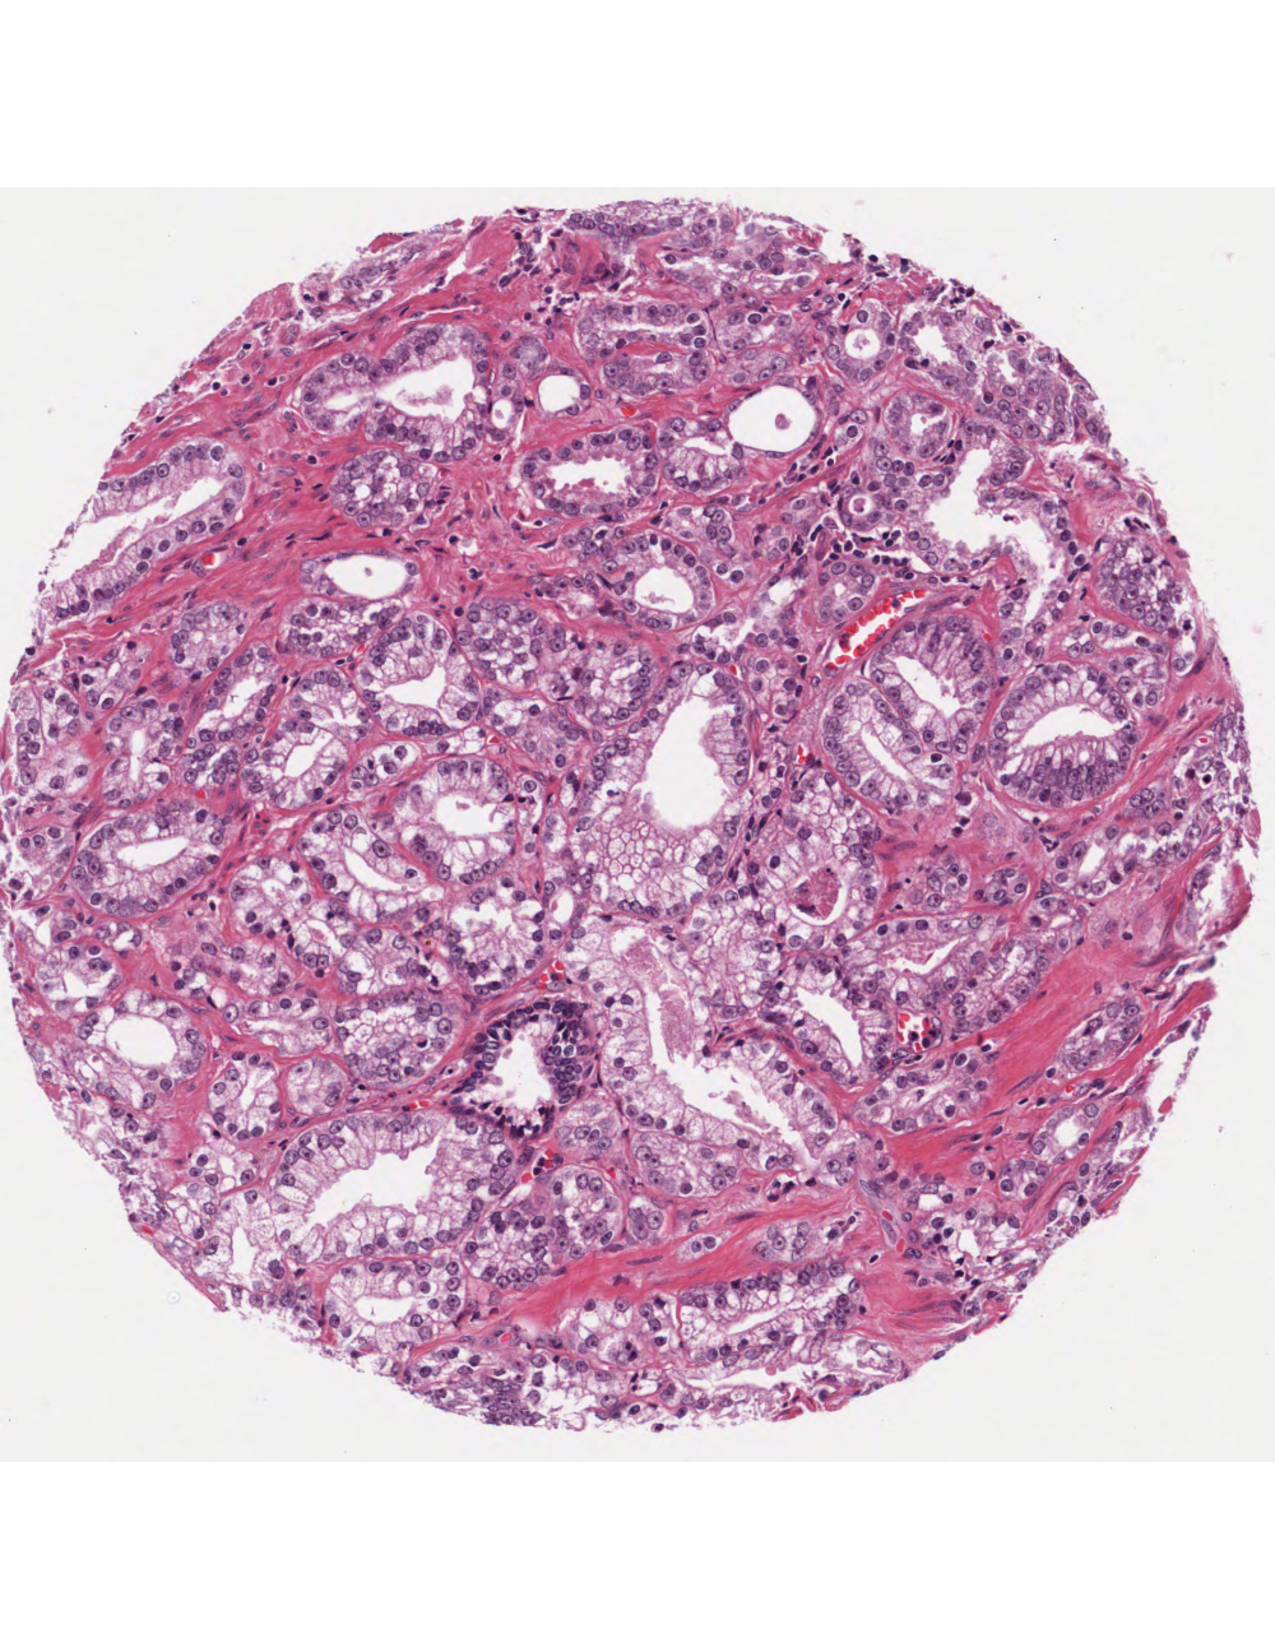
\includegraphics[width=2.0cm]{figs/109_red.pdf}
\caption{Stained tissue images in the dataset}
\label{fig:TissueImageExample}

\end{figure}  
  

The dataset has a nearly even split among the classes with 76 images belonging to `cancerous' class and remaining 73 `non-cancerous'. Another point to note over here is that the tissues in these images were stained in two separate batches, so the dataset may not be indicative of the variability in staining. Note that this dataset is significantly bigger than the datasets used in other works - indeed \cite{naik2007gland} uses a dataset of 44 images for their approach.


\subsection{Results}
In this section, we discuss the results for the different features we extract from the images. The classifiers we try out on the extracted features are 
\begin{itemize}
\item Support Vector Machine with Gaussian Kernel (\textbf{\texttt{SVM}})
\item K-nearest neighbor classifier (\textbf{\texttt{KNN}})
\item Decision Tree classifier (\textbf{\texttt{DTREE}})
\end{itemize}
For each of these classifiers, 10-fold cross-validation was performed. The results are summarised in Table~\ref{table:accuracy}. As can be seen from the table, SVM classifier with lumen and epithelial features performs the best, resulting in an accuracy of 81.2\%. Further, the LocalMinima technique of finding the epithelial features works the best. 

\begin{table}
\centering
\begin{tabular}{|c|c|c|c| }
\hline
 & \textbf{\texttt{SVM}} & \textbf{\texttt{KNN}} & \textbf{\texttt{DTREE}} \\ \hline
\textbf{\texttt{LocalMin}} & 81.2\% & 69.8\% & 71.8\% \\ \hline
\textbf{\texttt{kMeans}} & 71.8\%  & 66.4\% & 59.1\% \\ \hline
\textbf{ \texttt{HoughTrans}} & 77.9\% & 73.2\% & 70.5\% \\ \hline
\end{tabular}
\caption{\label{table:accuracy}Accuracies of different approaches}
\end{table}

The ROC curves for local minima (\textbf{\texttt{LocalMin}}), Elliptical (\textbf{\texttt{kMeans}}) and Hough transform (\textbf{\texttt{HoughTrans}}) based features are shown in Figures~\ref{fig:ROC_localMin},\ref{fig:ROC_kMeans} and \ref{fig:ROC_circleConv} respectively. The area under curve further shows effectiveness of our approach. 

 

\begin{figure}
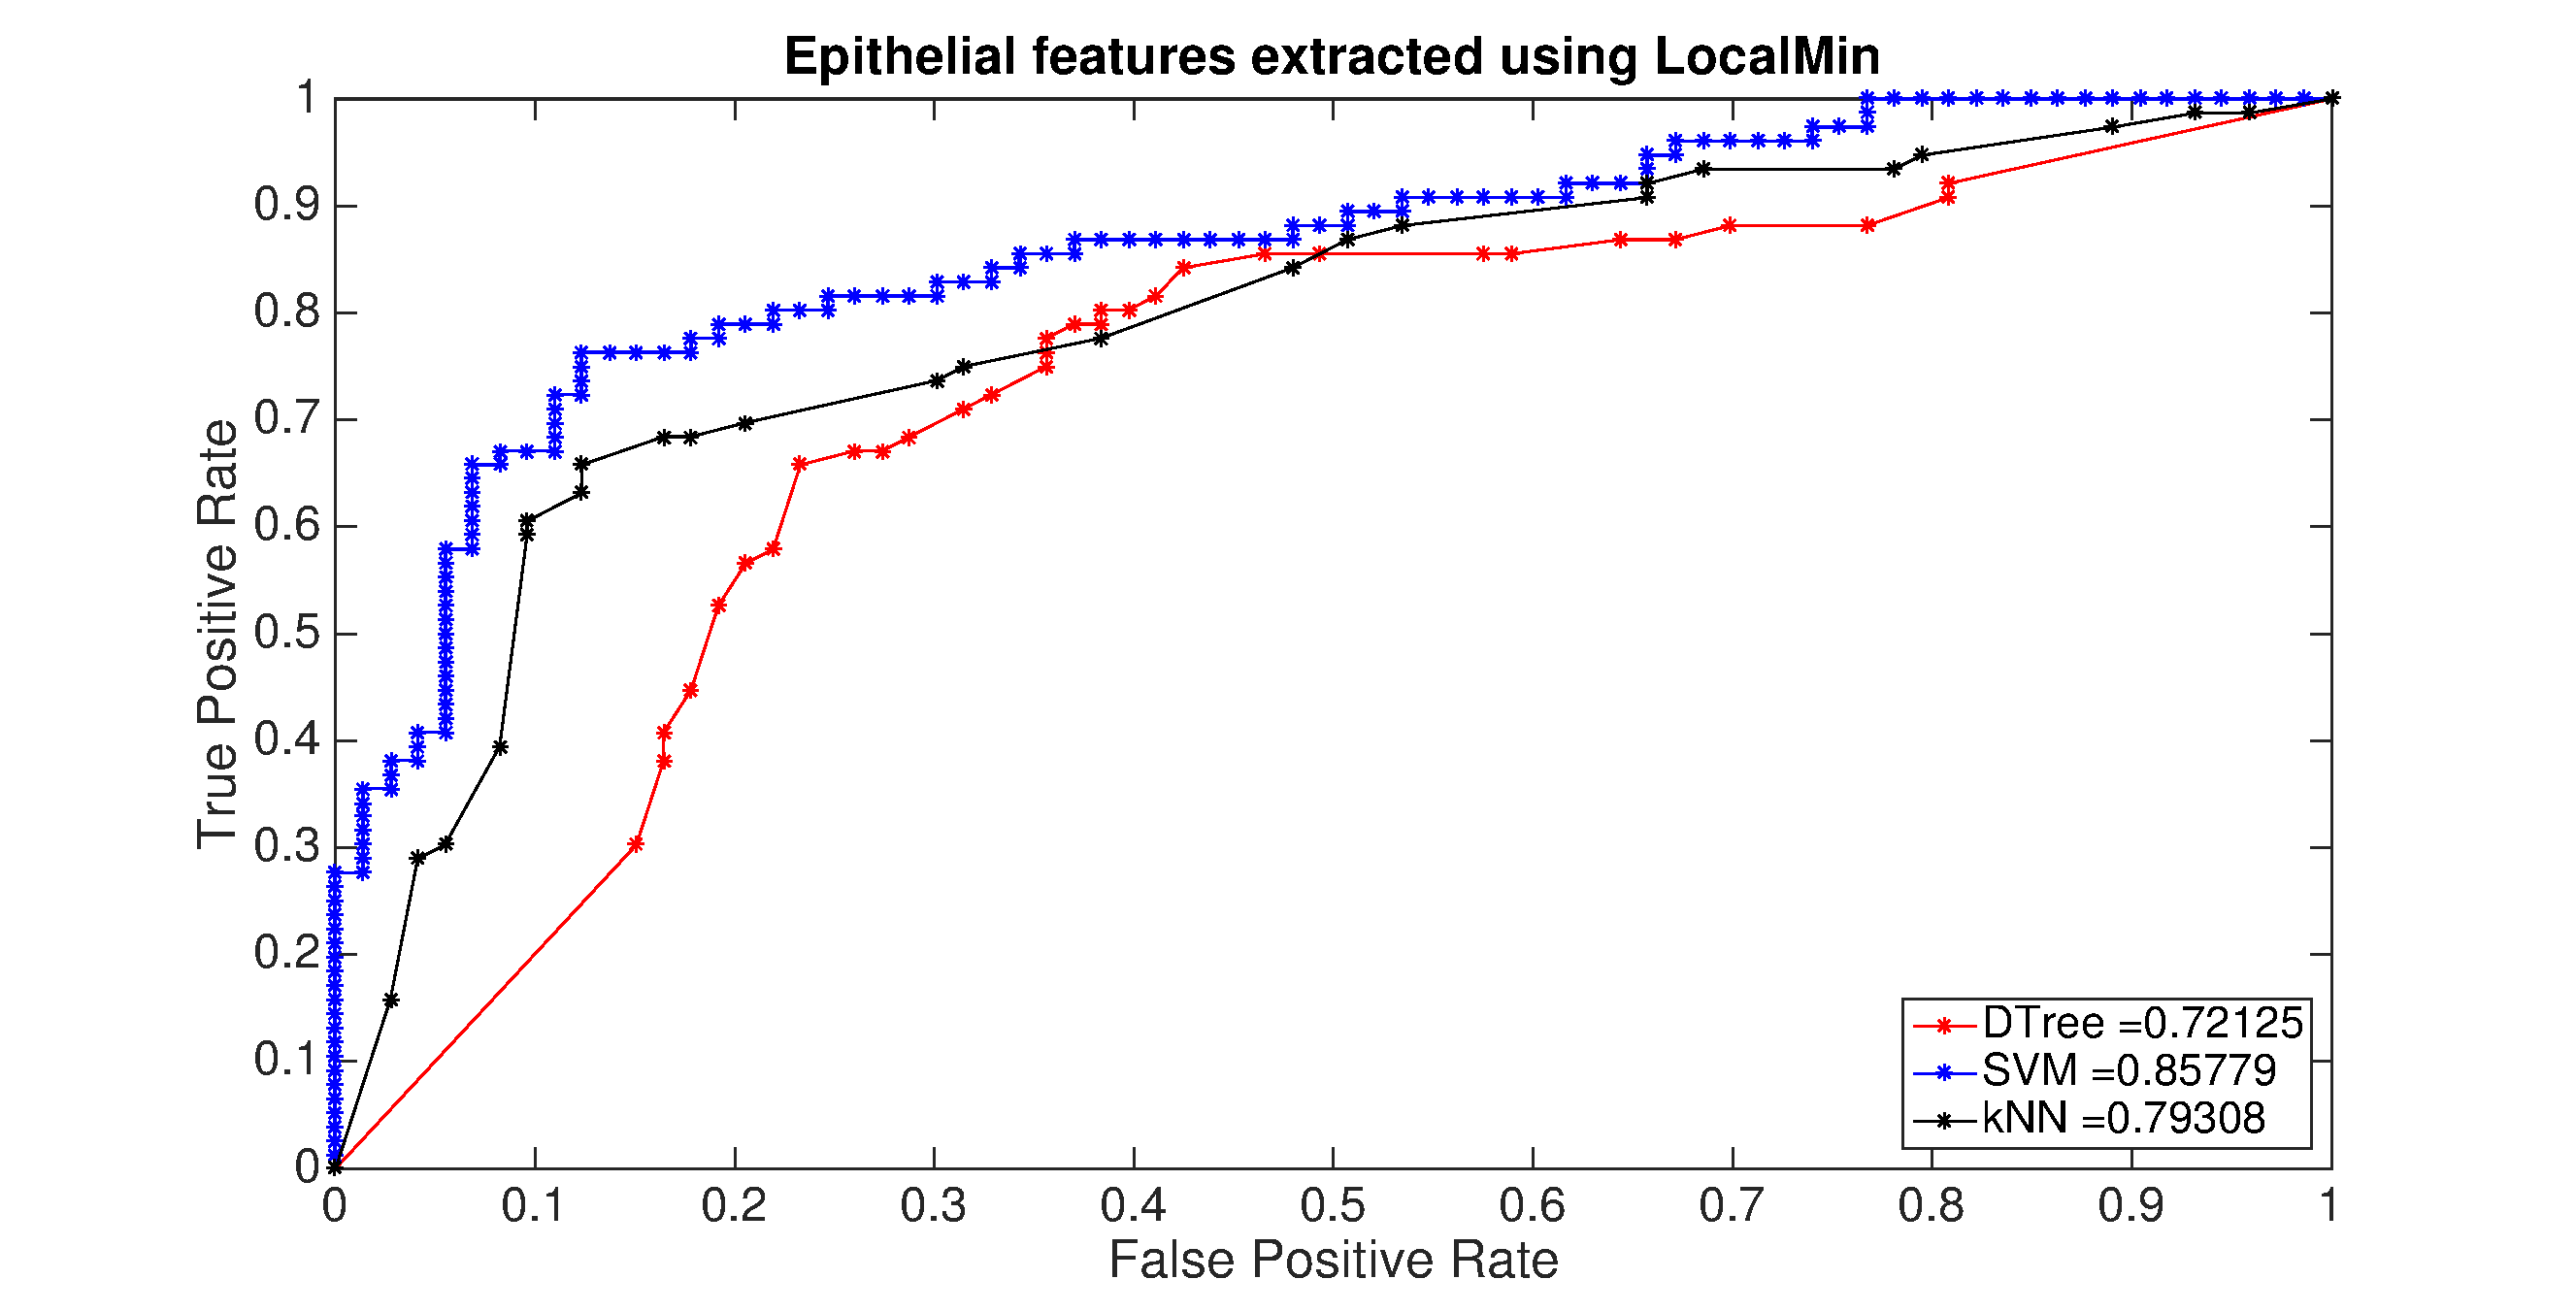
\includegraphics[scale=0.2]{figs/ROC_localMin.pdf}
\caption{\label{fig:ROC_localMin}ROC curve for local minima based epithelial based features}
\end{figure}  

\begin{figure}
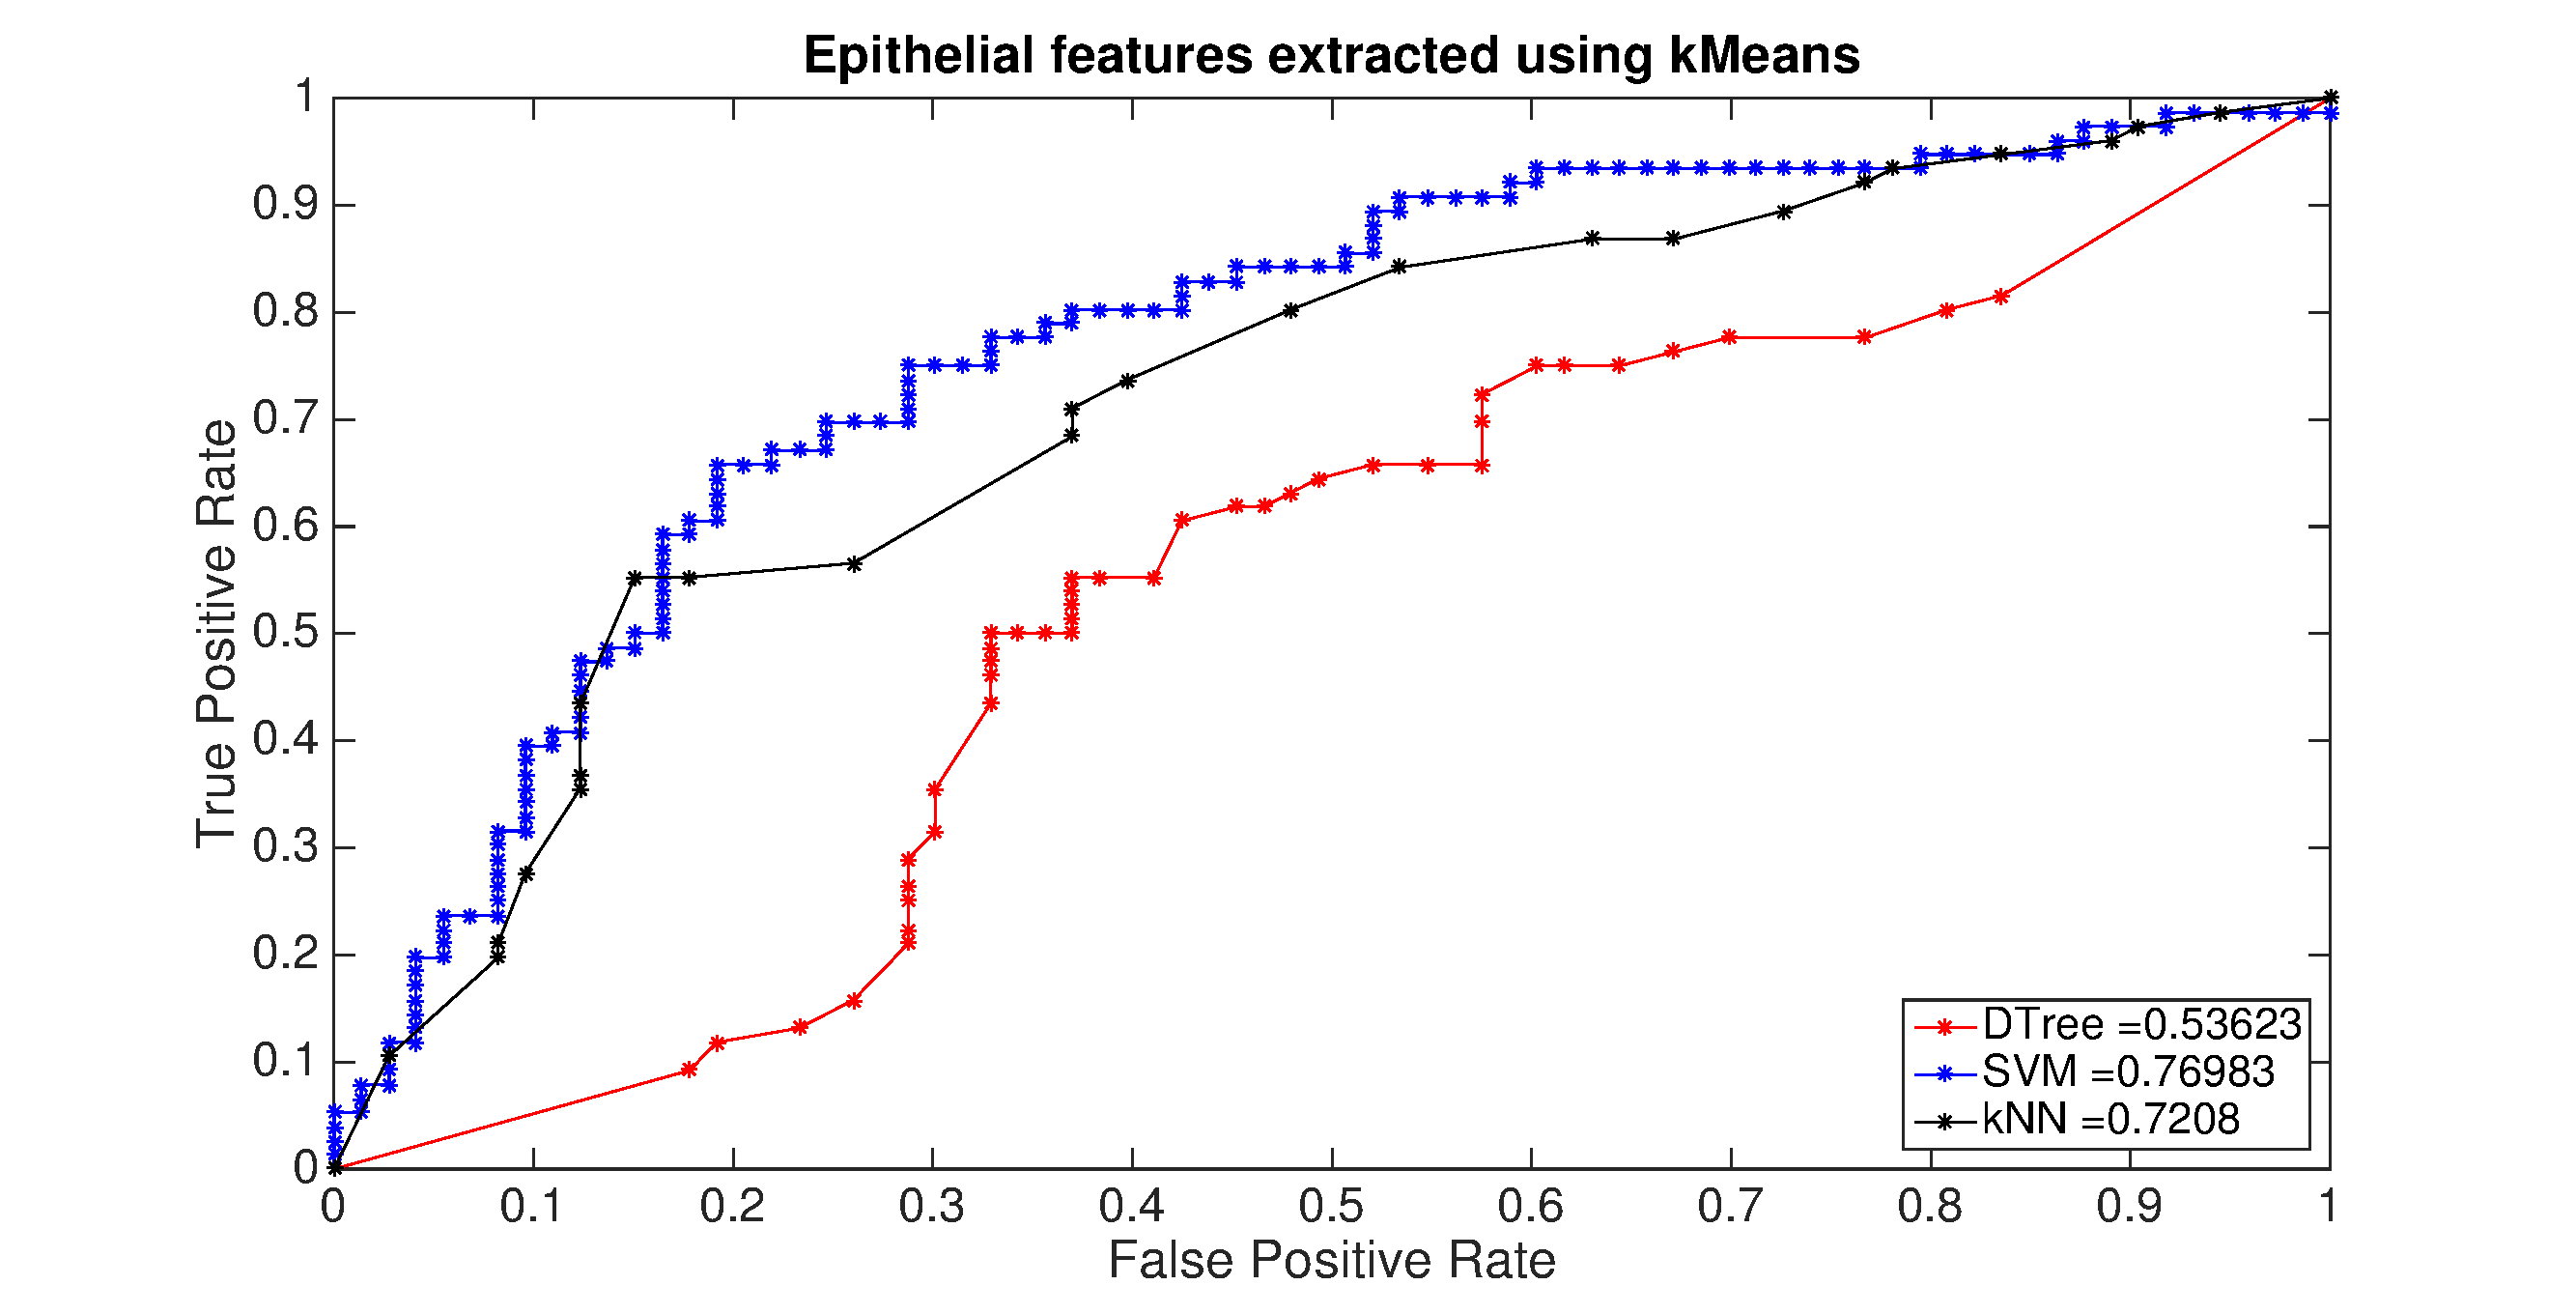
\includegraphics[scale=0.2]{figs/ROC_kMeans.pdf}
\caption{\label{fig:ROC_kMeans}ROC curve for k-means based epithelial based features}
\end{figure}


\begin{figure}
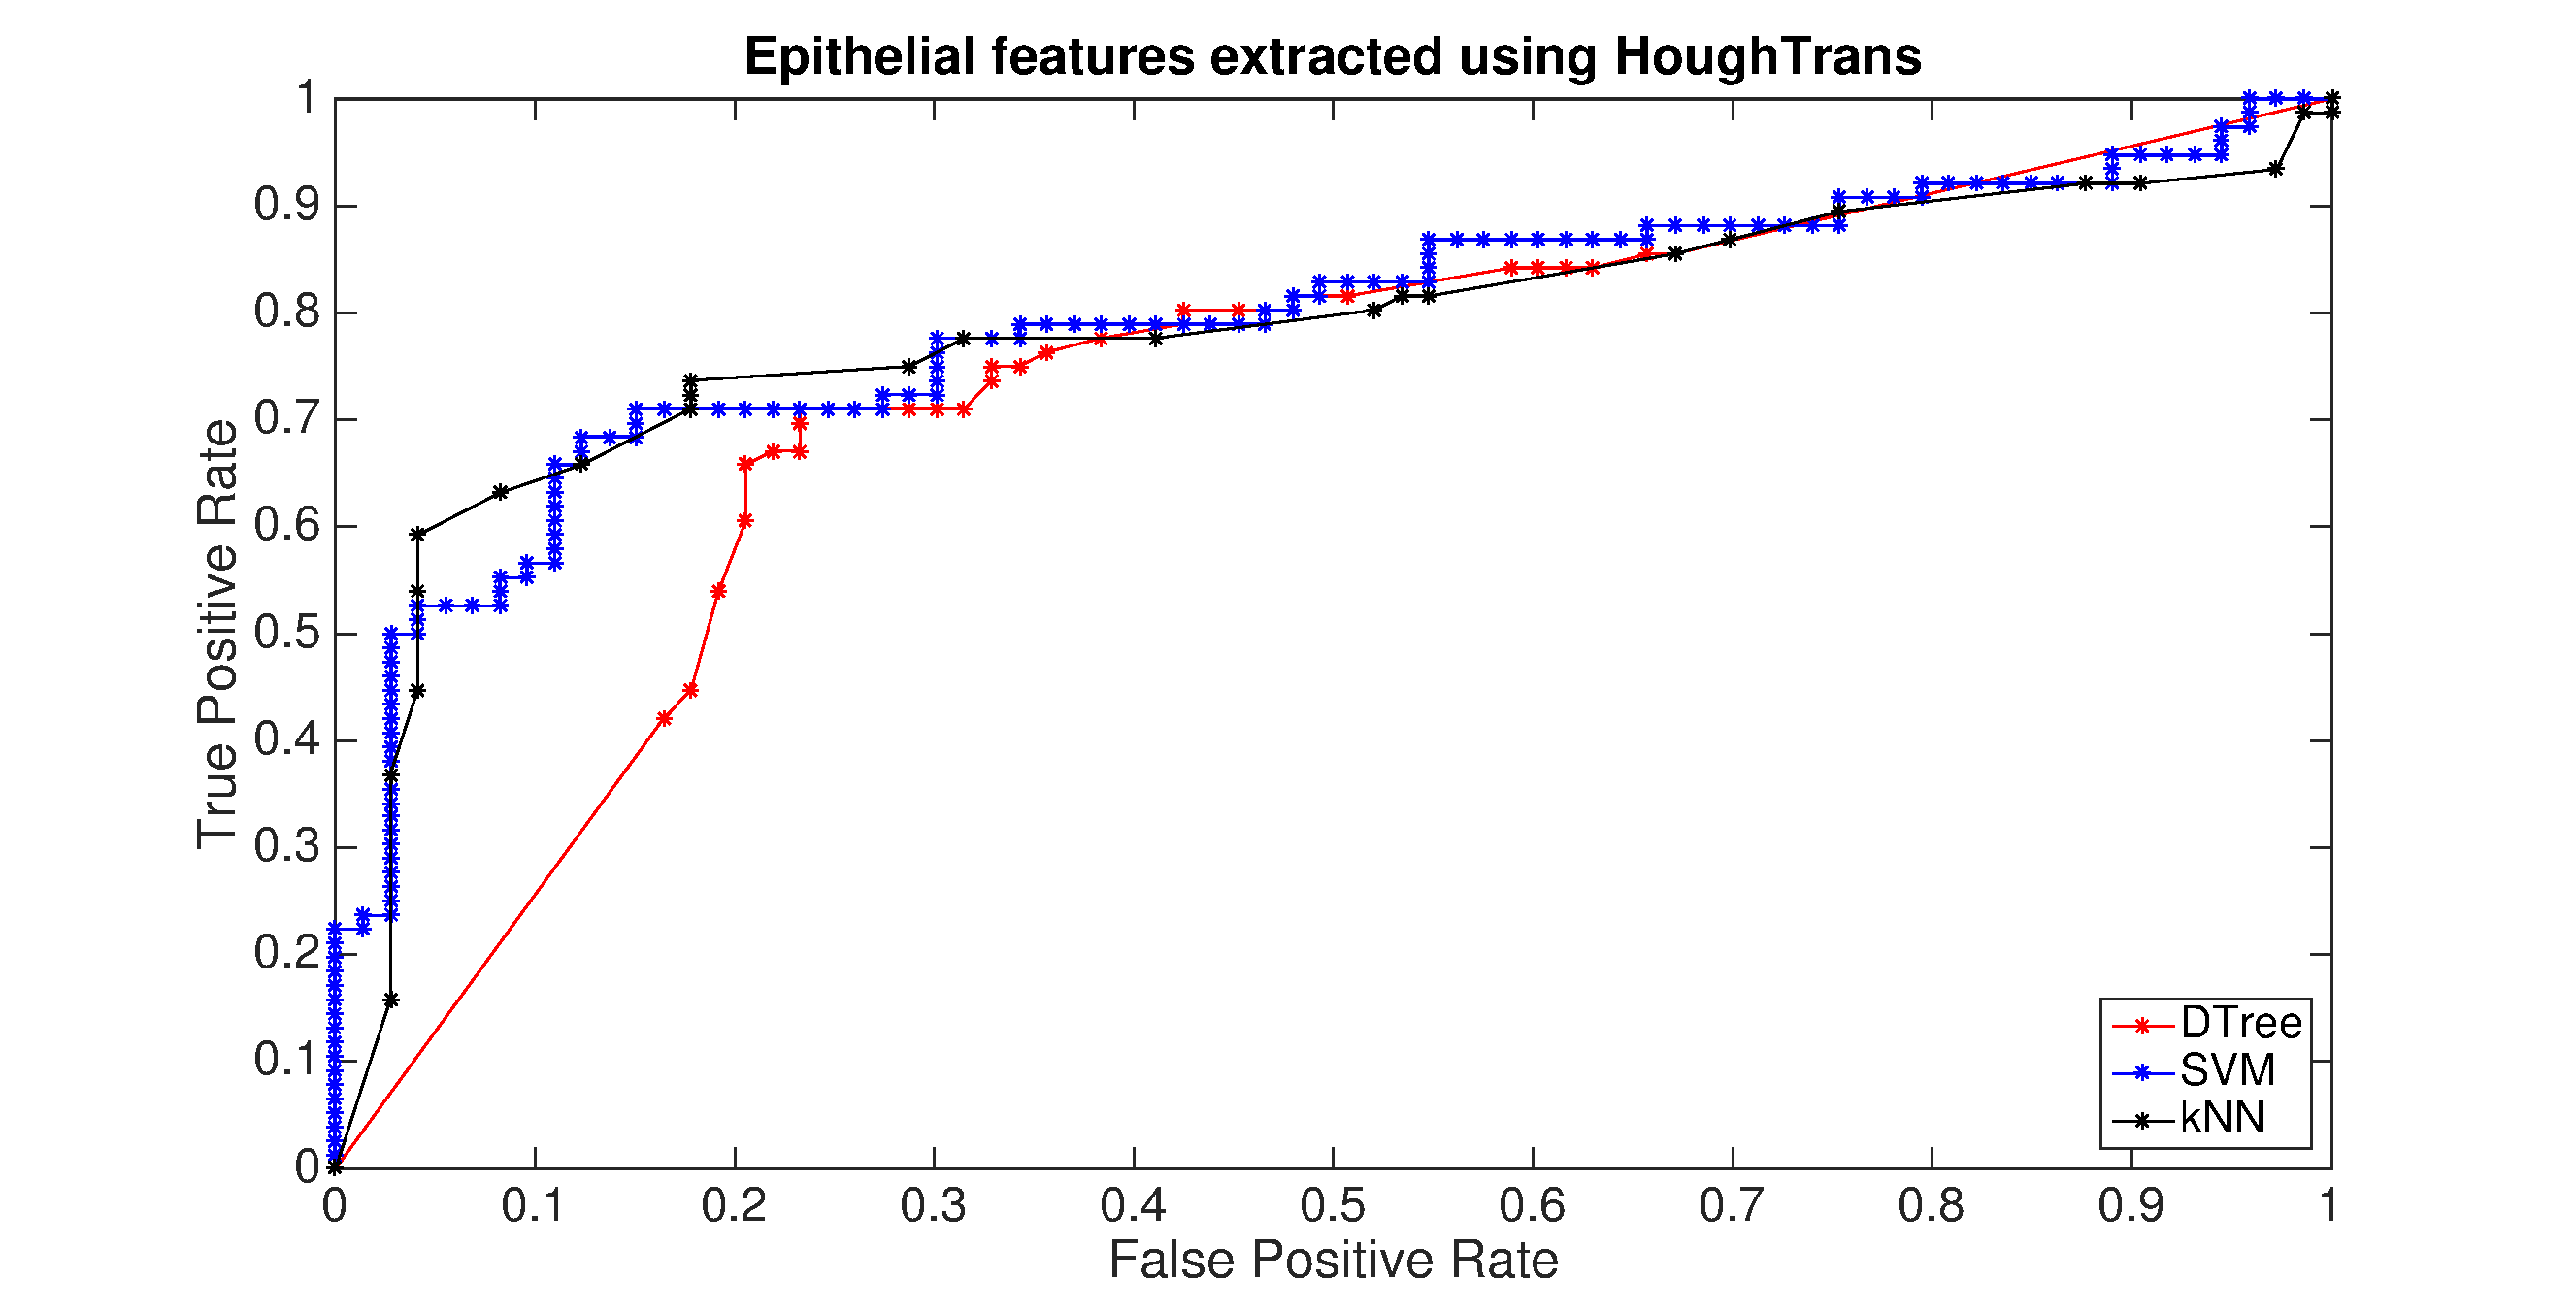
\includegraphics[scale=0.2]{figs/ROC_circleConv.pdf}
\caption{\label{fig:ROC_circleConv}ROC curve for Hough Transform based  epithelial features}
\end{figure} 



Finally, we also note the precision and recall obtained for detecting cancer in these images using local minima based epithelial features with SVM classifier. Our approach has a high recall of 86.4\%, and a reasonable recall of 75\%.

\begin{table}
\centering
\begin{tabular}{|c|c|c|c| }
\hline
 & \textbf{\texttt{SVM}} & \textbf{\texttt{KNN}} & \textbf{\texttt{DTREE}} \\ \hline
\textbf{Precision} & 86.4\% & 71.8\% & 68.7\% \\ \hline
\textbf{Recall} & 75\% & 73.7\%  & 75\% \\ \hline
\end{tabular}
\caption{\label{table:PrecisionRecall}Precision and Recall Values for different classifiers when epithelial features are extracted based on local minima technique}
\end{table}